\documentclass[11pt]{article}

\usepackage[margin=1in]{geometry}
\usepackage{amsmath}
\usepackage{booktabs}
\usepackage{graphicx}
\usepackage{microtype}
\usepackage[hidelinks]{hyperref}

\title{SnapReady: A Webcam Coach for Passport Photos\\[0.2em] \large CIS 5810 Final Project Proposal (Option 1)}
% \author{Yincheng Zhou, Teammate 2, Teammate 3}
\date{}

\begin{document}
\maketitle
\vspace{-2.5em}

SnapReady helps a person take a valid passport photo with a webcam. The input is live video of a real person. The output is a $600 \times 600$ photo (2 $\times$ 2 in) that follows the US passport rules. Instead of rejecting a bad photo afterwards, SnapReady tells the user the one thing to fix right now, and takes the photo by itself once everything passes. It is built from existing modules (MediaPipe, OpenCV) in three pieces: check, guide, finish.

\section{Pipeline}

Every webcam frame (1280x720, about 30 fps) goes through MediaPipe's Face Landmarker, which gives 478 landmarks, blink scores and head pose. From these we compute 11 measurements (Table~\ref{tab:rules}) and compare each to a rule. The first failing rule, in a fixed order, becomes the one instruction on screen. When all rules pass for 20 frames in a row, we keep the sharpest of those frames and finish it.

\paragraph{Check} Distance uses the pinhole model (Lecture 1): the iris is about 11.7\,mm for almost every adult, so distance $= f \cdot 11.7\,\text{mm} / \text{iris width in pixels}$. We want at least 50\,cm, since a close lens makes the nose look about 30\% wider~\cite{ward2018}. Sharpness is the variance of the Laplacian (HW1).

\paragraph{Guide} Each rule is a simple limit on one measurement, e.g.\ head turned at most 19$^\circ$ either way. Intuition: five problems at once is confusing, so we only show the first failing one, big moves first (distance, position), then head, eyes, light and blur.

\paragraph{Finish} A similarity transform (Lecture 5) levels the eyes and scales the head to 60\% of the height (spec: 50--69\%). The person is then blended onto white with a Laplacian pyramid (Project 3).

\begin{table}[h]
\centering
\footnotesize
\begin{tabular}{@{}lll@{}}
\toprule
Measurement & How we compute it & Rule in v1 \\
\midrule
distance, face height & iris width (pinhole), chin to forehead & $\ge 50$\,cm, $\ge 0.20$ of height (by hand) \\
offset x, y & face center minus image center & $|x| \le 0.11$, $-0.04 \le y \le 0.13$ \\
head turn, nod & MediaPipe face transform & $|\text{turn}| \le 19^\circ$, $-11^\circ \le \text{nod} \le 10^\circ$ \\
head tilt & line between the eye corners & $|\text{tilt}| \le 11^\circ$ \\
eye closure & max of the two blink scores & $\le 0.17$ \\
brightness, shadow & median gray of face; bright half / dark half & 68 to 194; $\le 1.29$ \\
sharpness & Laplacian variance of the face crop & $\ge 3.25$ \\
\bottomrule
\end{tabular}
\caption{Measurements and rules. Limits not marked ``by hand'' are fitted on data.}
\label{tab:rules}
\end{table}

\vspace{-1.5em}
\section{Data, baseline and results}

\paragraph{Data} No dataset labels webcam photo mistakes, so we made test cases. LFW~\cite{lfw}: 600 people, each photo damaged a little (should pass) and a lot (should fail) in position, blur, exposure, side shadow and rotation. Pointing'04~\cite{pointing04}: 4650 head poses, bad if turned or nodded over 15$^\circ$. Open/closed eyes~\cite{eyesdata}: 900 AI faces. Half of each set fits the limits by grid search, the other half is the test. Metric: balanced accuracy, the mean of bad caught and good passed (50\% = guessing).

\paragraph{Baseline} Viola-Jones Haar cascades~\cite{viola2001} for face and eyes, plus whole-image brightness and sharpness. Head turn and nod cannot be measured, so they are 0. It gets the same rule fitting as v1.

\paragraph{SnapReady (v1)} MediaPipe's Face Landmarker~\cite{mediapipe}, measuring inside the face outline. It wins 5 of 7 checks (Table~\ref{tab:results}).

\begin{table}[h]
\centering
\footnotesize
\begin{tabular}{@{}lccccccc@{}}
\toprule
 & Centered & Sharp & Exposure & Even light & Head level & Facing & Eyes open \\
\midrule
Baseline (Viola-Jones) & \textbf{99.4} & \textbf{90.2} & 88.6 & 78.2 & 74.0 & 78.8 & 77.0 \\
v1 (MediaPipe)         & 96.2 & 87.4 & \textbf{94.9} & \textbf{81.1} & \textbf{79.7} & \textbf{90.5} & \textbf{100.0} \\
\bottomrule
\end{tabular}
\caption{Balanced accuracy (\%) on the test half.}
\label{tab:results}
\end{table}

\vspace{-1.5em}
\paragraph{Limits} The baseline wins centering because LFW was centered by the same Haar detector. We don't know yet why it wins sharpness. Eyes at 100\% is too optimistic: a real smiling face gets ``Open your eyes'' (Fig.~\ref{fig:guide}h). A soft side shadow passes (d), and the segmenter can keep a second person (Fig.~\ref{fig:passport}). So far the app only ran on a simulated clip, not live with people.

\begin{figure}[h]
\centering
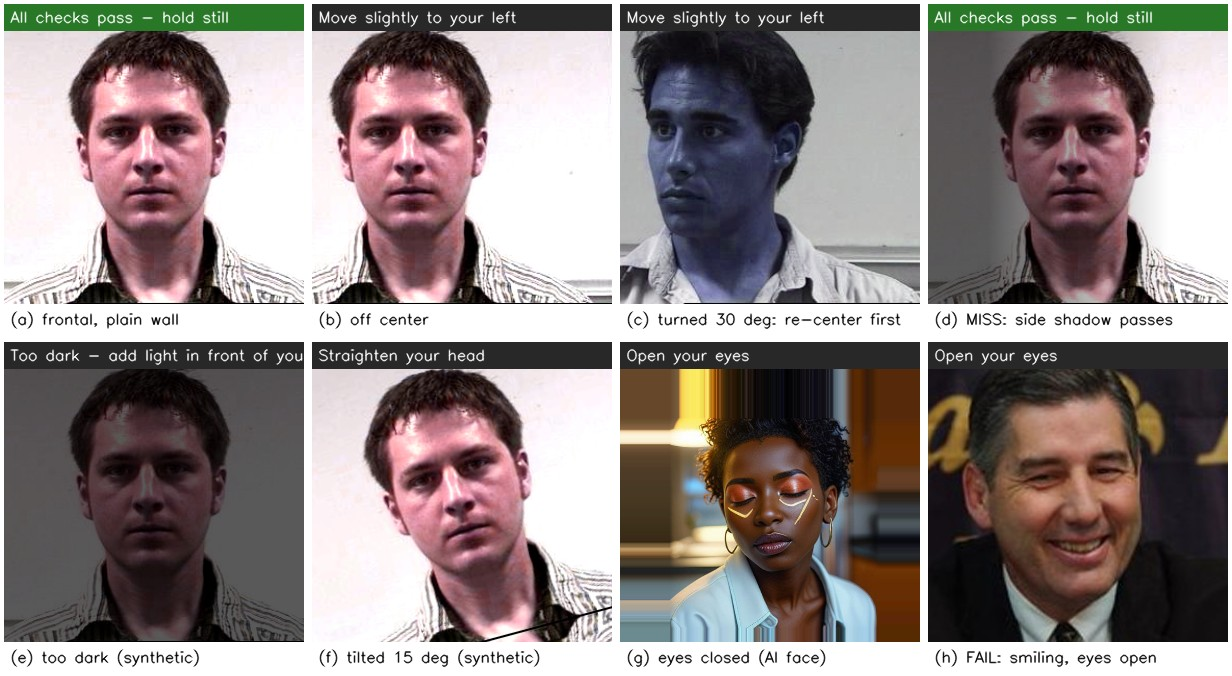
\includegraphics[width=0.8\linewidth]{figures/guidance.jpg}
\caption{The banner is the instruction v1 shows. (d) and (h) are failures.}
\label{fig:guide}
\end{figure}

\vspace{-1em}
\begin{figure}[h]
\centering
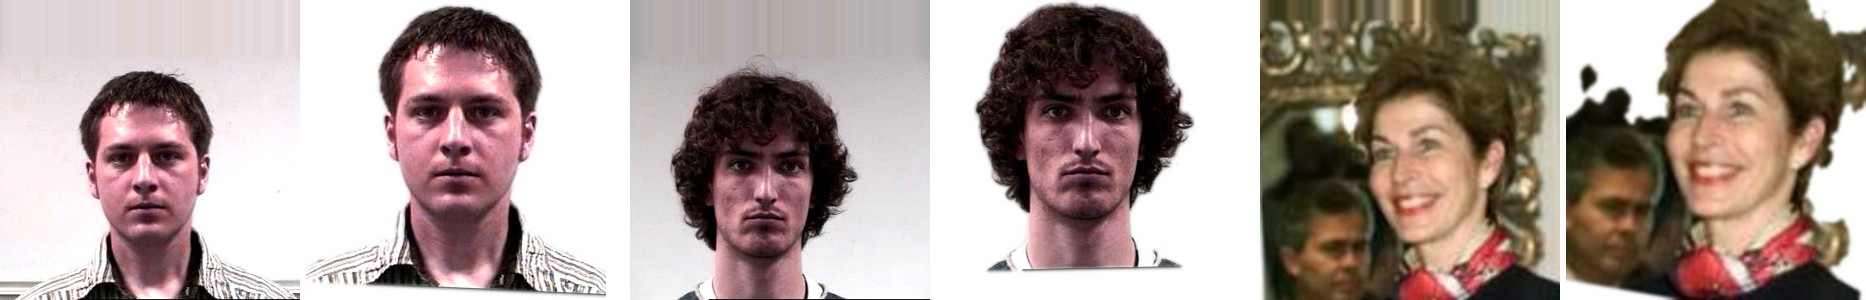
\includegraphics[width=0.9\linewidth]{figures/passport.jpg}
\caption{Input and finished photo. The last one fails: the person behind is kept.}
\label{fig:passport}
\end{figure}

\vspace{-1.5em}
\section{Plan}
\begin{itemize}
    \setlength{\itemsep}{0pt}
    \item \textbf{Midterm.} (2) Record our own webcam test set with scripted mistakes and refit the limits. (3) Fix eyes vs smiling with eyelid landmarks. (4) Re-test centering on Pointing'04 and blur on real motion blur.
    \item \textbf{Final.} (5) Keep only the person connected to the face. (6) Check head size and eye line of every output against the spec. (7) User study: time to a valid photo, SnapReady vs normal camera.
\end{itemize}

\paragraph{Credits and AI use} MediaPipe Face Landmarker and Selfie Segmenter (Apache 2.0), OpenCV Haar cascades; no training. \texttt{benchmark.py} reproduces every number. We used Claude Code (Anthropic) to help write the code and draft this proposal.

{\footnotesize
\begin{thebibliography}{9}
\setlength{\itemsep}{0pt}
\bibitem{viola2001} P. Viola, M. Jones. Rapid object detection using a boosted cascade of simple features. CVPR 2001.
\bibitem{mediapipe} Y. Kartynnik et al. Real-time facial surface geometry from monocular video on mobile GPUs. CVPRW 2019.
\bibitem{lfw} G. Huang et al. Labeled Faces in the Wild. UMass Tech. Report 07-49, 2007.
\bibitem{pointing04} N. Gourier et al. Estimating face orientation from robust detection of salient facial features. ICPRW 2004.
\bibitem{eyesdata} M. Mlodawski. closed-open-eyes. huggingface.co/datasets/MichalMlodawski/closed-open-eyes.
\bibitem{ward2018} B. Ward et al. Nasal distortion in short-distance photographs: the selfie effect. JAMA Facial Plast. Surg. 2018.
\end{thebibliography}}

\end{document}
